%-------------------------------------------------------------------------
\section{DPRT Method}
Classic PRT  is a physically-based rendering method to accelerate on-line computations of the (simplified) \textit{Rendering Equation}:
\begin{align}
L(\bm{\omega}_0 ) &= 
\int_{\Omega}   L_{\epsilon}(\bm{\omega}_i ) 
\underbrace{f(\bm{\omega}_i,\bm{\omega}_0) 
V(\bm{\omega}_i) H_N(\omega_i) }_{T(\bm{\omega}_i,\bm{\omega}_0) }
\,  \, d\bm{\omega}_i , 
\label{rendering equation PRT}
\end{align}
where $L_{\epsilon}$ accounts for all incoming radiance over the hemisphere, $f$  describes the surface reflectance properties $f$ (BRDF), $H_N$ is the \textit{Lambert's Law} and $V$ the \textit{Visibility Function} describing geometric information of the scene.\\
It precisely exploits the essence of static/non-deformable objects by uniquely determining the integrand $T(\bm{\omega}_i,\bm{\omega}_0)$ (called the \textbf{\textit{Transfer Function}} ), which contains the costly-to-compute  \textit{Visibility} term,
\begin{align*}
V :  \mathcal{S}  \times \Omega \rightarrow \{0,1\} \quad,
\end{align*}
for each surface point $\bm{s} \in \mathcal{S} \subset \mathbb{R}^3$ \cite{CohenBook}. 
\\
Both functions $L_{\epsilon} $ and $T$  are projected onto a suitable set of orthonormal basis functions for faster evaluation of the \textit{Rendering Equation} \ref{rendering equation PRT}. 
For $m$ number of coefficients of the basis functions and $l_i$, $t_i$ being the $i$-th coefficient of $L_{\epsilon} $ and $T$ respectively, equation \ref{rendering equation PRT} reduces to \cite{sloan2002precomputed} 
\begin{align}
L(\bm{\omega}_0 ) \approx \sum_{j}^{m} l_j \cdot t_j 
\label{Eq: Reduced Rendering Eq}
\end{align}
We chose a \textit{Spherical Harmonics} (SH) bases to encode the Transfer Function $T$ and the light environment $L_{\epsilon}$.
\\
\\
 As mentioned above, our aim is to extend the PRT method to malleable and dynamic objects, but avoiding costly pre-computations and storage of every single \textit{Transfer Function} $T_i$ per shape query $S_i$ (with $i \in [1,2,\dots, d]$ and $d$ : $\#$ deformations ). \\
With this in mind, we suggest a data-based model, a fully Convolutional Neural Network, to infer the \textit{Transfer Function} $T_i$, more precisely the coefficients of its SH-encoding $t_j$'s, for any given shape query $S_i$.
This makes the costly ray-casting computations superfluous and solves the abusive memory requirements, only necessitating the storage of the network's parameters. 
%%%%%%%%%%%%%%%%%%%%%%%%%%%%%%%%%%
% -------------- GEOMETRY IMAGE ----------------- 
%%%%%%%%%%%%%%%%%%%%%%%%%%%%%%%%%%
\subsection{Data: Geometry Images}
We propose learning directly \textbf{on} the object's surface in order to leverage its underlying shape structure. \textit{Geometry Images} present an planar shape representation on which standard 2D CNNs can be applied \cite{gu2002geometry, sinha2016deep}. 
\\ 
Surfaces with a single boundary (topological disks) are mapped onto a unit square and later discretized (or resampled) into a regular grid of $n \times n$ vertices. 
For simplicity, but without loss of generality of our method, we  chose a \textit{Harmonic Map}, based on \cite{HarmonicMapping}, for the parametrisation of the interior of the 2D-grid. 
\begin{figure}[H]
  \centering
    \includegraphics[width=0.5\textwidth]{Figures/Geo_image}
     \caption{GeoImage}
     \label{Fig: GeoImage}
\end{figure}
It is to note that we apply deformations only on the reconstructed object (right shape of Figure (\ref{Fig: GeoImage}) ) in order to make our shape representation, \textit{Geometry Images}, invariant to deformations. By doing so, we maintain a one-to-one pixel correspondence; hence, filtering out deformation invariant information of the surface; and therefore, facilitating the feature extraction of surface properties that are more correlated to self-shadowing. 
\\
The surface information we transform into \textit{Geometry Images} to use as regressor for the CNN are: vertex positions $\mathcal{P}$ and normals $\mathcal{N}$. 
\begin{align*}
	\mathcal{P} = [ P_x, P_y, P_z ]^T , \quad
	\mathcal{N} = [ N_x, N_y, N_z ] ^T 
\end{align*}
with  $P_i, N_i \in \mathbb{R}^{n \times n }$ being the position and normal images, respectively, for each coordinate $i \in \{ x,y,z\}$.
\\
\\
Resulting, our CNN model predicts a corresponding sequence of \textit{Geometry Images} $\mathcal{T}$,
\begin{align*}
	f_{CNN} (  \mathcal{P} , \mathcal{N} ) = \mathcal{T} 
\end{align*}
consisting of the SH-coefficients of the \textit{Transfer Function} of the input shape, as introduced above (see eq. \ref{Eq: Reduced Rendering Eq}):
\begin{align*}
	\mathcal{T} = [ t_1, t_2, \dots, t_m ]^T \in \mathbb{R}^{m \times n \times n} 
\end{align*}
that is, vertex $i$ of image $t_j$ represents the transfer coefficient $j$ of vertex $i$ of the input surface.
\\
Figure \ref{Fig: Method_Overview} illustrates the basic procedure of the method.
\begin{figure}[h]
  \centering
    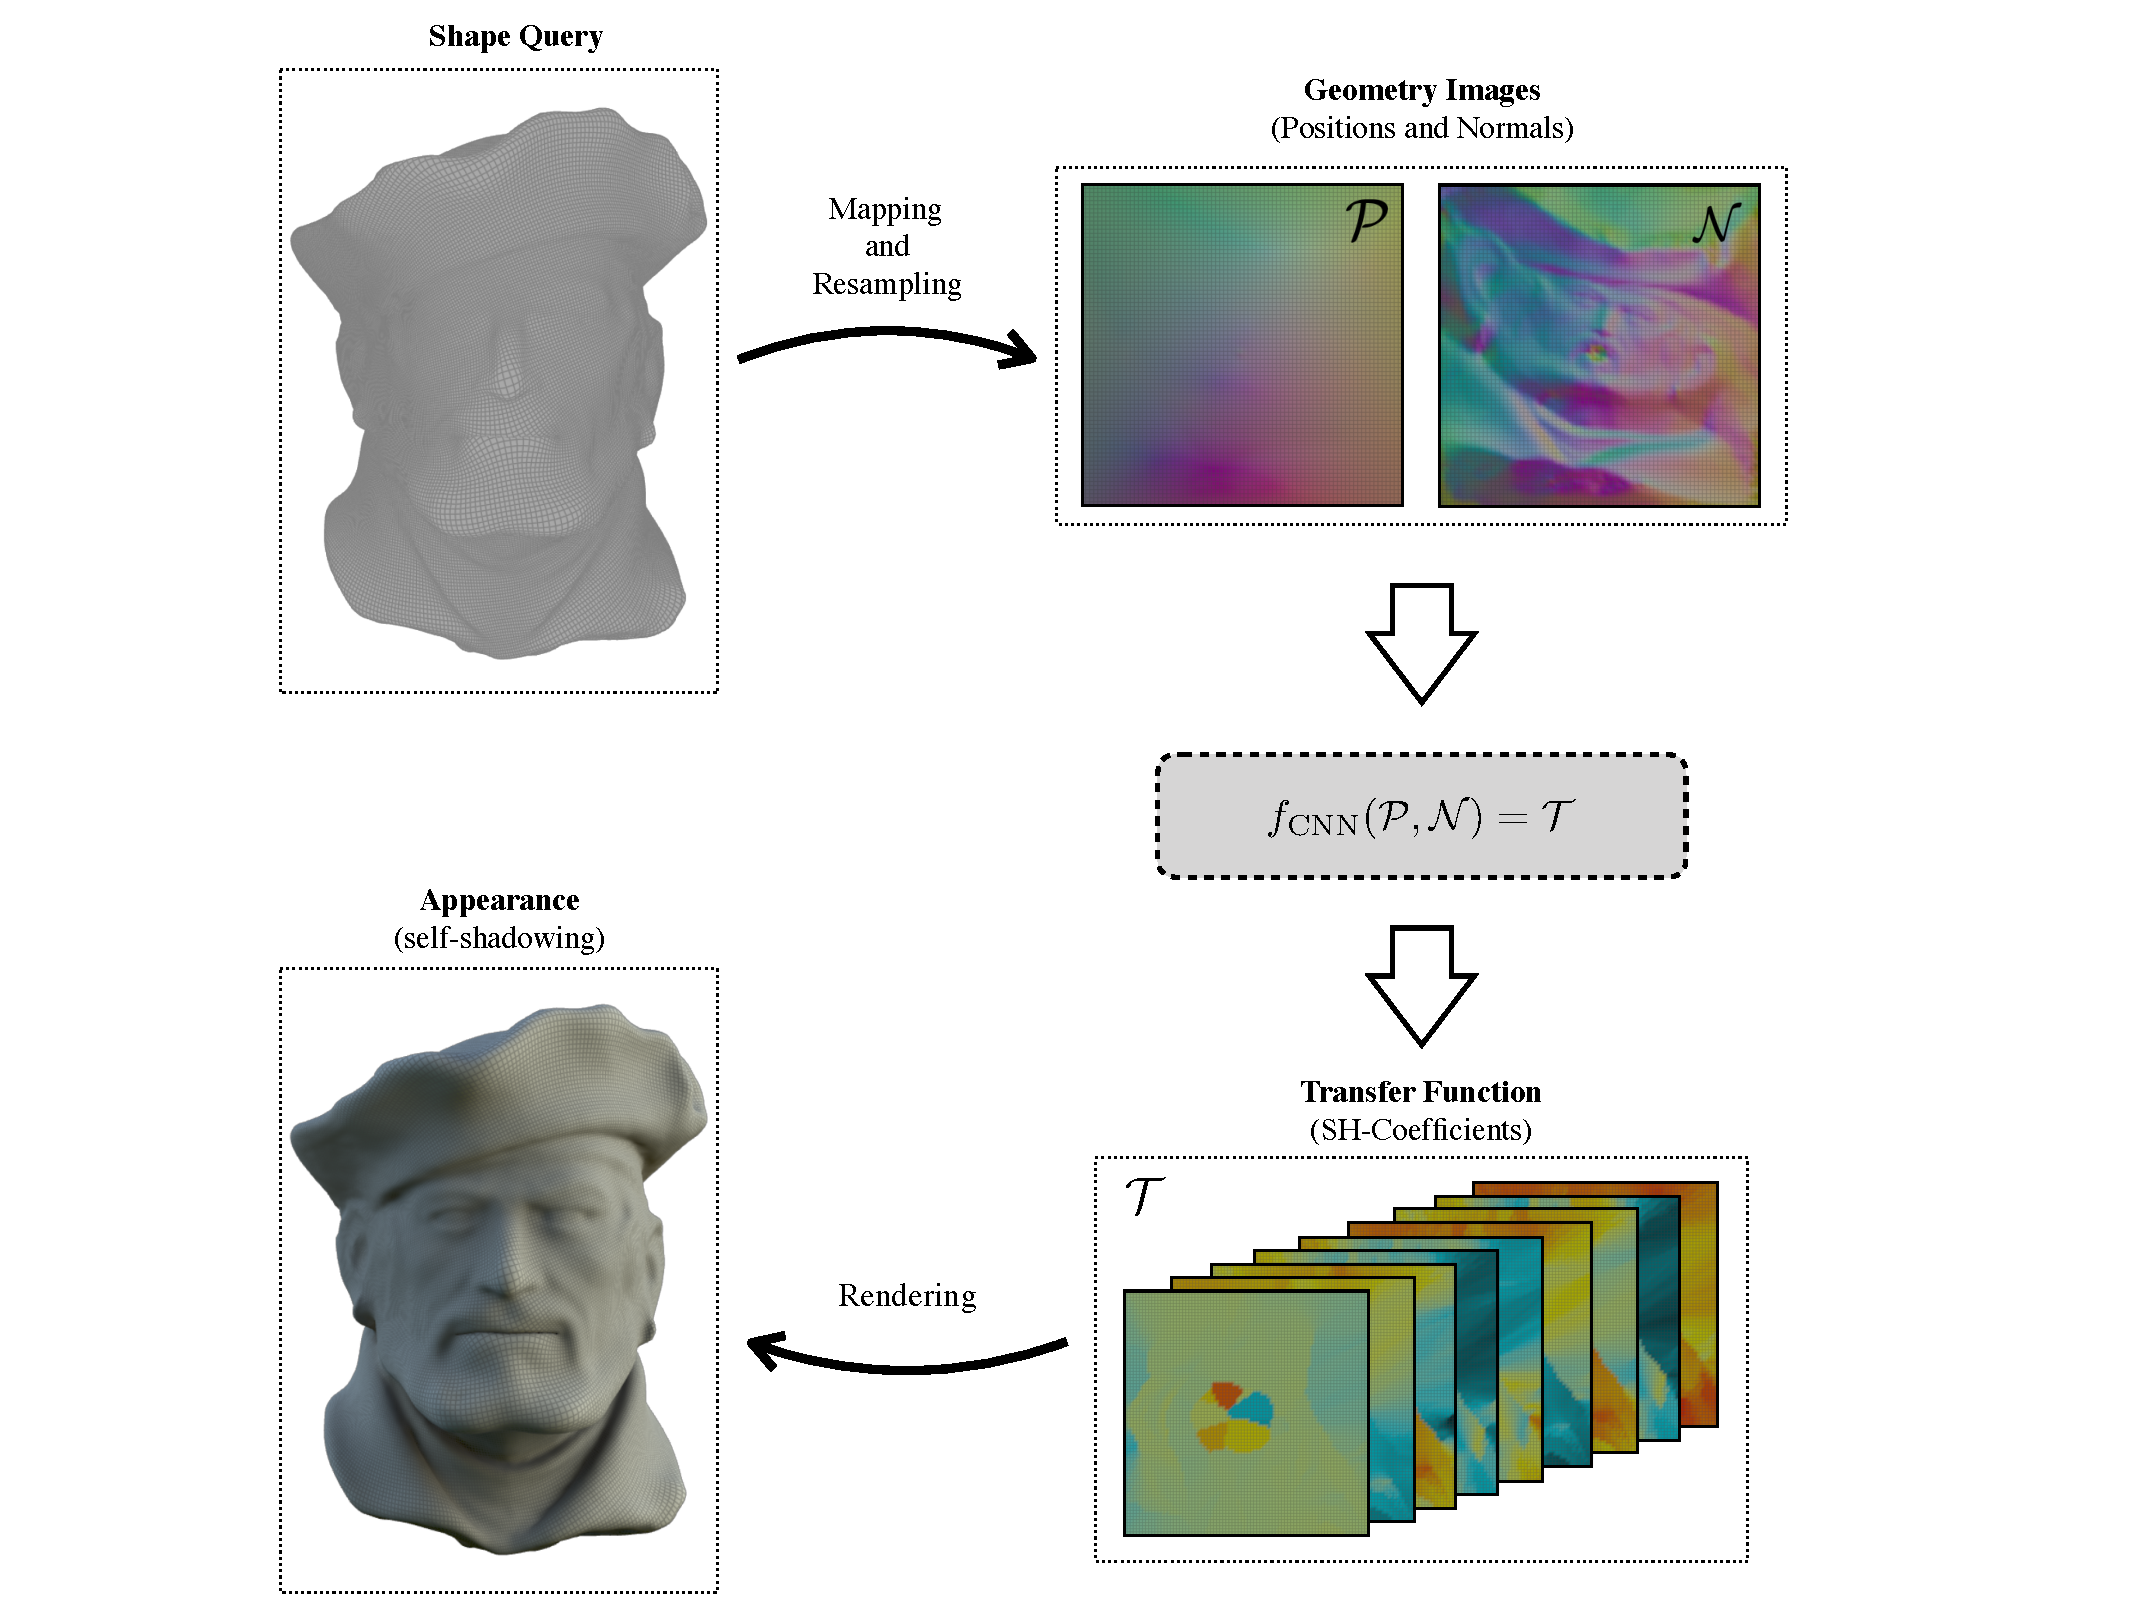
\includegraphics[width=0.5\textwidth]{Figures/Overview_method.pdf}
     \caption{Method Overview}
     \label{Fig: Method_Overview}
\end{figure}
%%%%%%%%%%%%%%%%%%%%%%%%%%%%%%%%%%
% -------------- NETWORK ----------------- 
%%%%%%%%%%%%%%%%%%%%%%%%%%%%%%%%%%
\subsection{ Network Architecture and Training}
In order to DPRT to function for real-time rendering scenarios, it requires very fast network inference times. However, to achieve high accuracies, existing deep convolutional network models rely on very deep architectures with millions of parameters, consequently being computationally expensive and memory intensive, and therefore becoming impractical for real-time application. \\
However, it has been extensively shown that most neural network models are highly compressible and can be significantly accelerated, eventually making them deployable to devices with low memory resources and applicable to real-time environments \cite{Deep_Compression, Survey_NN_Compression}.
\\
However, the topic of \textit{network optimisation} reaches beyond the scope of this work. Here, we will make use of a classic deep CNN architecture to to demonstrate the main principles of our method. In section [??] we show that even neglecting network compression our DPRT-approach already achieves immense memory savings. 
\subsubsection*{Architecture: \\} 
The topology of our deep convolutional network consists of an encoder and decoder with skip connections based on \cite{U-Net}. Both encoder and decoder consist of sequences of ResNet blocks \cite{ResNet} each comprising a series of 2D-Convolution, Batch Normalisation, Down-sampling and ReLU - Activation layers (illustrated in Figure (\ref{Fig: NetworkTopology}) ). For the last layer of the decoder we use a Sigmoid-Activation-Function. Instead of a Pooling-Layer we perform down-sampling by increasing the stride, by a factor of two, within a Convolutional layer \cite{StridingConv}. To avoid information loss,  we make use of skip-connections, which passes outputs of encoding layers to the respective inputs of the decoding layers. The network has an approximate amount of $1,1 \cdot 10^7$ parameters. \\
\subsubsection*{Synthesis of Training Data :\\}
For a given object, we generate the training data by applying sequences of smooth deformations, obtained by a physically based or blendshape based animation (see Section ?? for examples), each of a total length of 500 frames. 
\\
For each frame $i \in [1,2,\dots,500]$ we store the position $\mathcal{P}_i$  and normal $\mathcal{N}_i$ images, and perform a full self-shadowing integration using ray-casting to compute and store the corresponding coefficients of the \textit{Transfer Function} $\mathcal{T}_i$ (ground truth).
\\
For most objects we chose an image resolution of $256 \times 256$. 
\subsubsection*{Training: \\} 
The network is trained on 450 samples, each consisting of six image channels of size $256 \times 256$. As cost function, we minimize the pixel-wise absolute error between predicted output and the ground-truth ($l_1$-loss), and the optimizer we use is ADAM \cite{ADAM}. 
\\
Convergence varies from object to object, but in most cases 500 to 1000 epochs are sufficient, using a batch size of 5. The network is implemented in Keras \cite{Keras} with Tensorflow as Backend. On a high-end GPU (NVIDIA GetForce GTX 2080) this takes around...(TO CHECK!)
%%%%
\begin{figure*}[t]
  \centering
    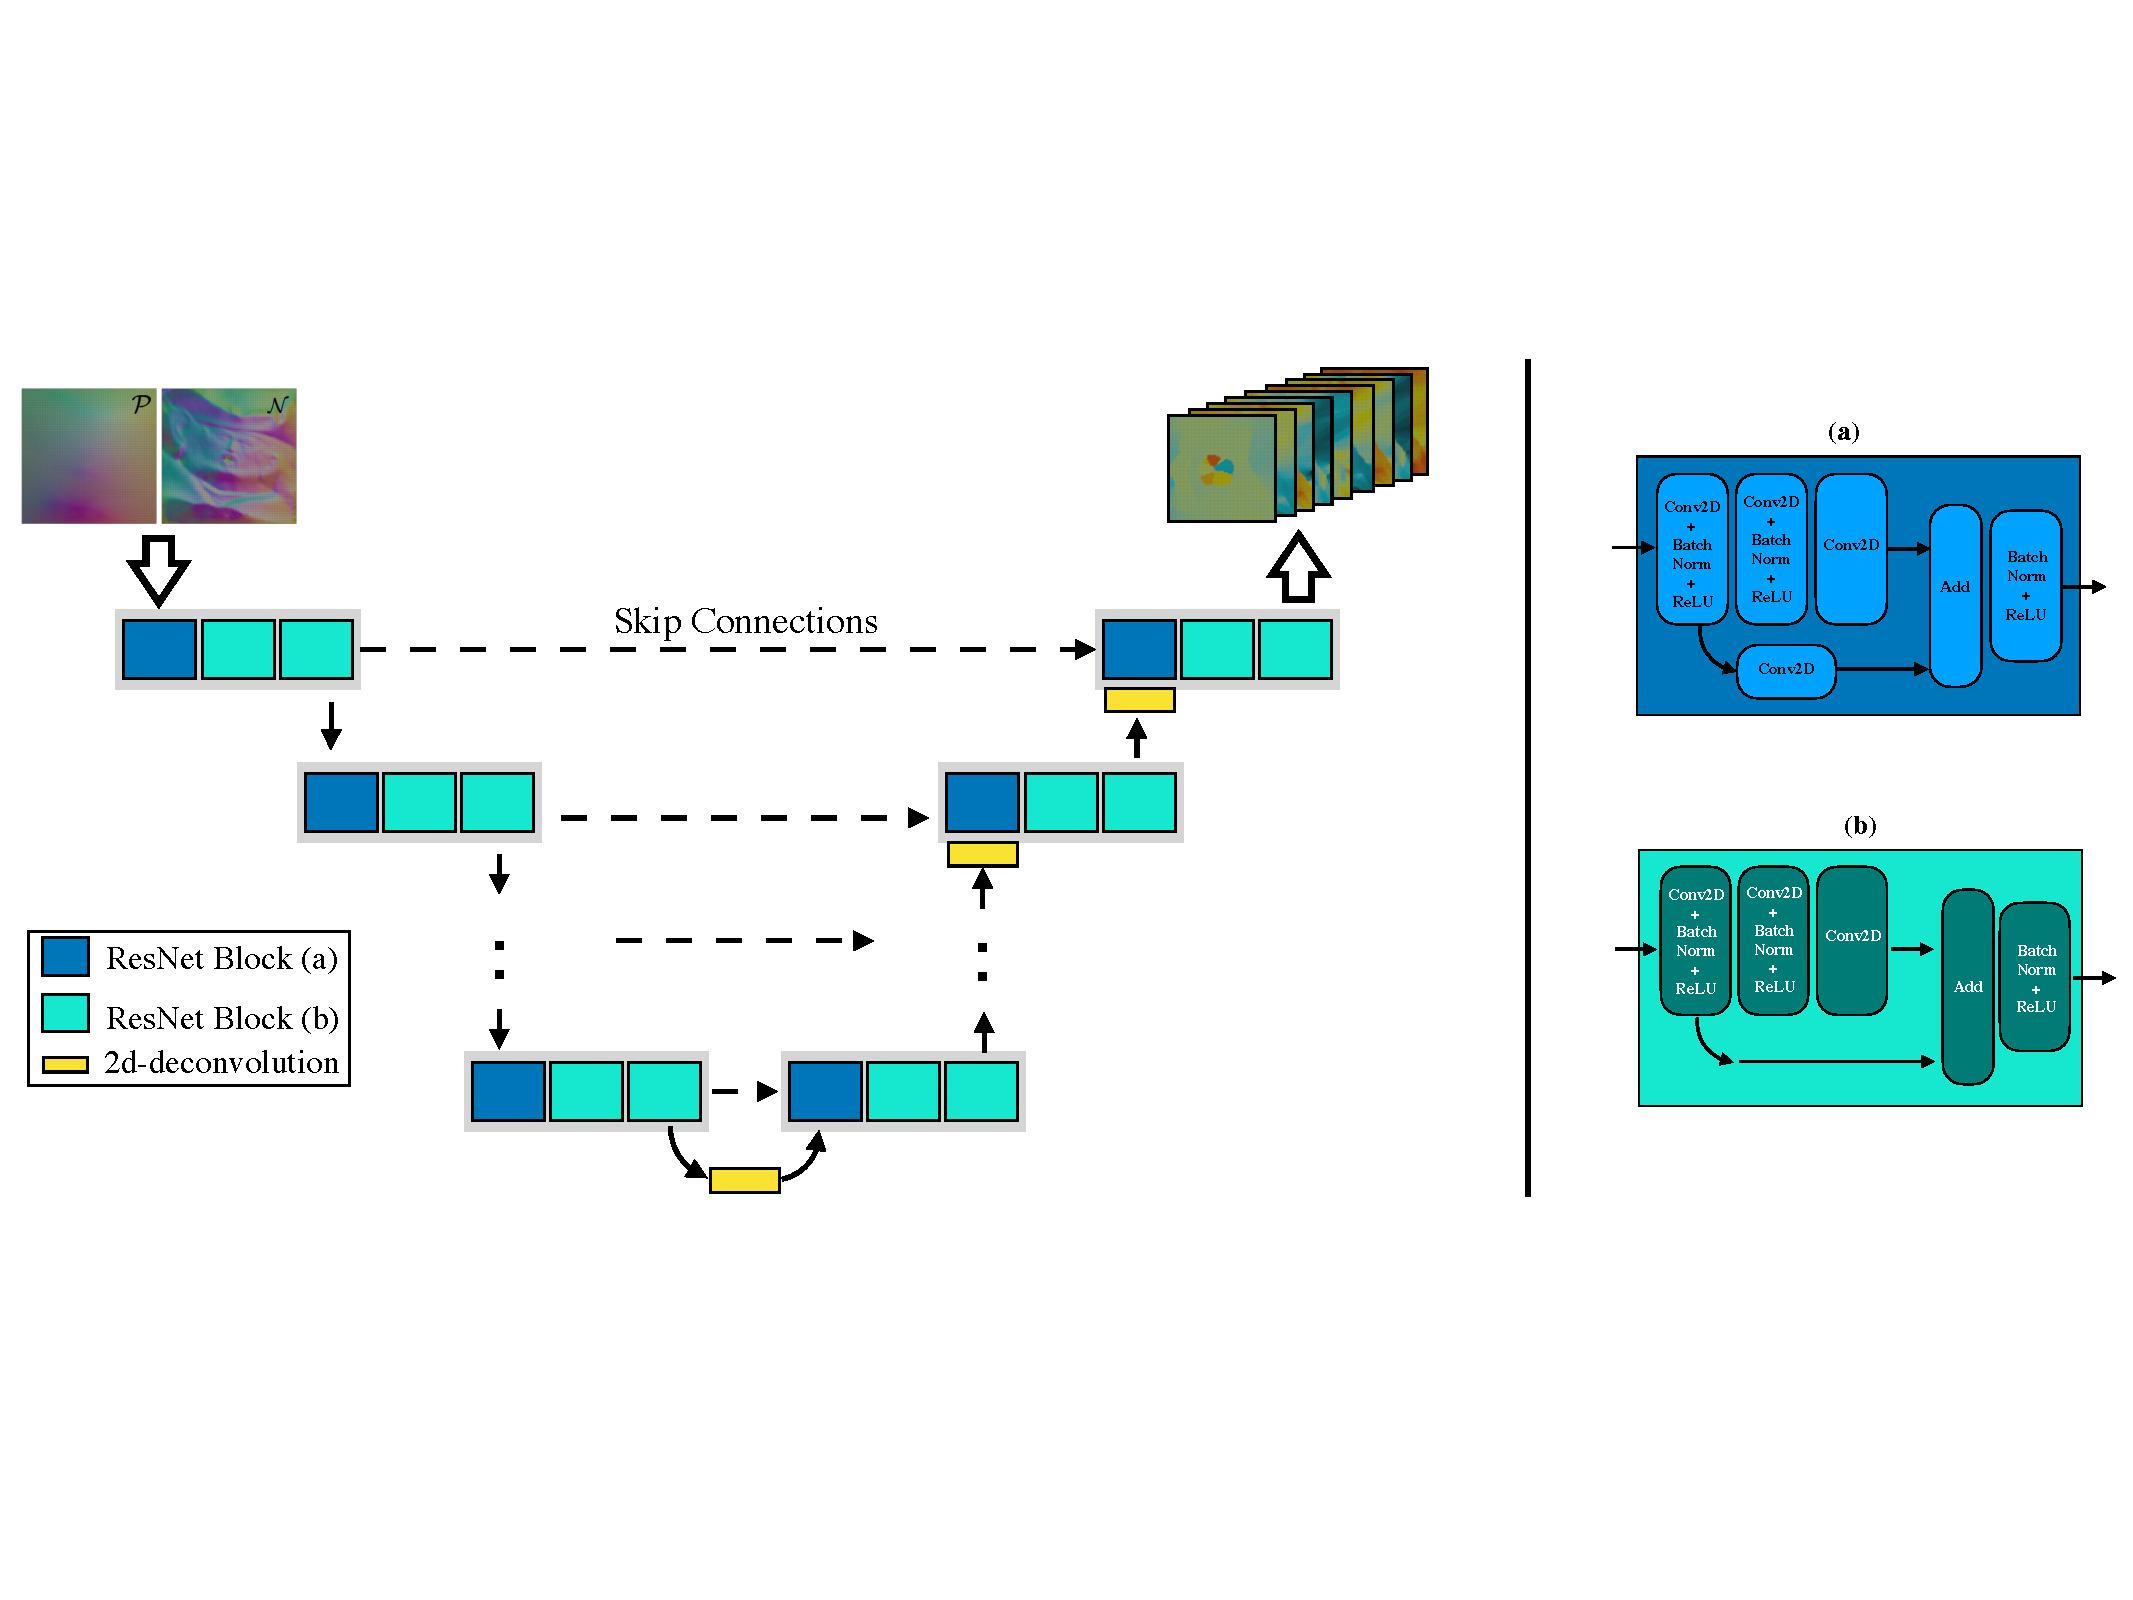
\includegraphics[width=0.7\paperwidth]{Figures/Network_topology.pdf}
     \caption{Network Topology}
     \label{Fig: NetworkTopology}
\end{figure*}

  


